\documentclass[twocolumn]{aastex701}

\usepackage{amsmath}
\usepackage{amssymb}
\usepackage{bm}
\usepackage{booktabs}
\usepackage{array}
\usepackage{url}
\usepackage{seqsplit}

\graphicspath{{figures/}}

\newcommand{\Rearth}{R_{\oplus}}
\newcommand{\Mearth}{M_{\oplus}}
\newcommand{\Searth}{S_{\oplus}}
\newcommand{\Teff}{T_{\rm eff}}
\newcommand{\Rgc}{R_{\rm GC}}
\newcommand{\LamEE}{\Lambda_{\rm EE}}
\newcommand{\LamHZ}{\Lambda_{\rm HZ}}
\newcommand{\fEE}{f_{\rm EE}}
\newcommand{\fHZ}{f_{\rm HZ}}
\newcommand{\HZcons}{{\rm HZ}_{\rm cons}}
\newcommand{\dd}{\mathrm{d}}
\newcommand{\ind}{\mathbf{1}}
\newcommand{\hashid}[1]{\texttt{\seqsplit{#1}}}

\shorttitle{A Conditional ExoEarth Projection in the 7--9 kpc Annulus}
\shortauthors{Jer\v{s}e}

\begin{document}

\hypersetup{
  pdftitle={A Posterior Model Projection of Narrow-domain ExoEarth Candidates in the Milky Way's 7--9 kpc Annulus},
  pdfauthor={Roman Jerse},
  pdfsubject={Posterior model projection of narrow-domain ExoEarth candidates around old G dwarfs}
}

\title{A Posterior Model Projection of Narrow-domain ExoEarth Candidates in the Milky Way's 7--9 kpc Annulus}

\author{Roman Jer\v{s}e}
\affiliation{Independent Researcher, Slovenia}
\email{}

\begin{abstract}
Kepler occurrence rates are defined per target star, whereas a Galactic
projection additionally requires an explicit host-star measure and a transport
assumption. We reconstruct the Bryson et al. Model~1 occurrence posterior from
the public DR25 inputs using corrected two-sided measurement-error propagation,
400 reliability/measurement realizations per completeness branch, and adaptive
ensemble Markov chain Monte Carlo. We propagate every retained posterior
realization through a pinned Just--Jahrei\ss/PARSEC host population. The target
is narrowly defined by $0.9\leq R_p/\Rearth\leq1.1$ and
$0.9\leq S_p/\Searth\leq1.1$, intersected with the present-day conservative
habitable zone, around operationally main-sequence $5300$--$6000$ K stars at
least 4.57 Gyr old in the $7$--$9$ kpc annulus. The host model gives
$N_\star=2.6306\times10^8$. The constant-completeness scenario yields median
$\langle\fEE\rangle=0.0123$ (68\% interval $0.0058$--$0.0235$) and
$\LamEE=3.22$ million ($1.52$--$6.19$ million). The zero-completeness scenario
yields $0.0174$ ($0.0080$--$0.0339$) and $4.57$ million
($2.10$--$8.91$ million), respectively. Both branches pass the declared
convergence and Monte Carlo error gates. However, the exact nominal DR25 target
contains zero candidates and zero summed catalog reliability, and more than
95\% of corrected catalog realizations also contain none. The reported
intervals therefore quantify the fitted posterior conditional on the adopted
separable occurrence model and frozen host model; they do not include local
support, occurrence-model-form, climate, host-population, or Galactic-transport
uncertainty. The result is a reproducible conditional model projection, not a
direct candidate-supported occurrence measurement and not a census of
habitable or inhabited worlds.
\end{abstract}

\keywords{Exoplanet astronomy --- Exoplanet population studies --- Habitable planets --- Milky Way disk --- G dwarf stars --- Astrostatistics}

\section{Introduction}\label{sec:intro}

The Kepler mission established that small planets are common and made
occurrence-rate inference central to exoplanet demography
\citep[e.g.,][]{Howard2012,Fressin2013,Petigura2013}. Modern analyses must
account for target selection, injection--recovery completeness, catalog
reliability, stellar-property uncertainties, and the functional form of the
underlying population \citep{Burke2015,ForemanMackey2014,Kunimoto2020}. These
issues are most severe for small planets at low instellation, where detections
are sparse and smooth models are extrapolated into weakly supported regions.

\citet{Bryson2021} formulated a differential occurrence model in planet
radius, instellation, and host effective temperature. Its output is a number
of planets per star. Converting that result into a Galactic population
expectation requires a second measure describing eligible stars and an
assumption that the Kepler-calibrated occurrence law can be transported to
that population.

Version~3 of this analysis implemented that transport with fixed median
parameter vectors. The present work replaces those plug-in values with a newly
reconstructed, corrected joint posterior; validates the host and TAMS
selection; audits direct DR25 support in the exact target; and freezes numerical,
model, climate, and spatial sensitivities before interpreting the result. The
constant- and zero-completeness treatments remain separate scenarios and are
never pooled into a confidence interval.

The demonstration intentionally answers a narrow astronomical question. It
does not infer inhabited planets, biospheres, continuously habitable worlds,
or complete physical Earth analogs. It estimates a radius--instellation
selection around an old, operationally defined G-star population within a
geometric Galactic annulus.

\section{Estimand and Nomenclature}\label{sec:estimand}

We define dimensionless planet radius and bolometric instellation as
\begin{equation}
 r\equiv\frac{R_p}{\Rearth},
 \qquad
 I\equiv\frac{S_p}{\Searth}.
 \label{eq:variables}
\end{equation}
A \emph{narrow-domain ExoEarth candidate} satisfies
\begin{equation}
 0.9\leq r\leq1.1,
 \qquad
 0.9\leq I\leq1.1,
 \label{eq:ee_box}
\end{equation}
and lies in the present-day conservative circumstellar habitable zone of its
host, evaluated with the $1\,\Mearth$ inner-boundary prescription of
\citet{Kopparapu2013,Kopparapu2014}. The modifier ``narrow-domain'' is
essential because ExoEarth has no unique radius convention across the
literature.

This definition does not determine planet mass, density, composition,
atmospheric state, surface water, geologic activity, magnetic field, or
biology. Radius alone is not a sufficient compositional classifier
\citep{Rogers2015}, and present-day habitable-zone membership does not imply
continuous residence in the zone.

Target hosts are thin- or thick-disk stellar assemblies satisfying
\begin{equation}
 5300\leq\Teff\leq6000\ {\rm K},
 \qquad
 t_\star\geq4.57\ {\rm Gyr},
 \label{eq:host_window}
\end{equation}
classified as main-sequence objects by Section~\ref{subsec:selector}, within
\begin{equation}
 7\leq\Rgc\leq9\ {\rm kpc}.
 \label{eq:annulus}
\end{equation}

$N_\star$ is the expected number of selected hosts. $\LamHZ$ is the expected
number of planets with $0.5\leq r\leq1.5$ in the present-day conservative HZ,
and $\LamEE$ is the expectation in Equation~(\ref{eq:ee_box}). These are
expected planets, not the probability that a star hosts at least one planet.
The result is conditional on
\begin{equation}
 \mathcal{M}=\{M_{\rm JJ},M_{\rm iso},M_{\rm TAMS},
 M_{\rm occ},M_{\rm HZ},D_R,Q_R\},
 \label{eq:model_stack}
\end{equation}
which denotes the Galactic model, isochrones, stellar selector, occurrence
model, climate prescription, radial domain, and quadrature.

\section{Host-Star Population}\label{sec:hosts}

\subsection{Generalized Just--Jahrei\ss\ model}

The host population is generated with the generalized Just--Jahrei\ss\ (JJ) Galactic disk model \citep{JustJahreiss2010,Sysoliatina2022}, pinned to commit \texttt{2828a2e8bfc3} (\texttt{jjmodel} v1.0.1; the full hash is given in Section~\ref{sec:data}). We use the pinned \texttt{tutorial2/parameters} and \texttt{sfrd\_peaks\_parameters} realization, the default four-slope broken-power-law IMF (\texttt{imfkey=0}), a solar Galactocentric distance of 8.17 kpc, and a runtime radial grid $4\leq R\leq14$ kpc with $\Delta R=0.5$ kpc. Only the thin and thick stellar disks are retained; the stellar halo is excluded.

Stellar assemblies are generated with the JJ-distributed Padova library based on PARSEC v1.2S tracks \citep{Bressan2012} and the associated PARSEC--COLIBRI isochrone generation \citep{Marigo2017}; the workflow downloads the multiband archive identified by DOI \href{https://doi.org/10.11588/data/ZCXHOE}{10.11588/data/ZCXHOE}. The COLIBRI extension is part of the library provenance but does not determine the selected main-sequence G-star rows. Each synthetic row $i$ at radial node $R_j$ carries a vertically integrated present-day surface-number weight $w_{ij}$ in ${\rm pc}^{-2}$.

The resulting host count is a JJ/PARSEC-conditioned expectation, not a direct Gaia census. The model is axisymmetric and vertically integrated; spiral arms and azimuthal substructure are not resolved. The sub-percent radial-grid diagnostic reported below is not a posterior uncertainty on $N_\star$: uncertainties in the JJ parameter realization, IMF, age--metallicity and star-formation prescriptions, and isochrone family are not propagated in this work.

\subsection{Operational main-sequence selector}\label{subsec:selector}

For each synthetic row, the stellar radius is reconstructed from current mass and surface gravity,
\begin{equation}
 \frac{R_{\star,ij}}{R_\odot}
 =\left[
 \frac{M_{f,ij}}{M_\odot}
 10^{\log g_\odot-\log g_{ij}}
 \right]^{1/2},
 \qquad \log g_\odot=4.438.
 \label{eq:rstar}
\end{equation}
The host indicator is
\begin{align}
 H_{ij}={}&
 \ind(d_{ij}\in\{\mathrm{thin},\mathrm{thick}\})
 \ind(5300\leq T_{ij}\leq6000)\nonumber\\
 &\times\ind(t_{ij}\geq4.57)
 \ind(\log g_{ij}<7)\nonumber\\
 &\times\ind\!\left[R_{\star,ij}\leq
 R_{\rm TAMS}(T_{ij})\right].
 \label{eq:host_indicator}
\end{align}
The final factor is the operational main-sequence classifier. The preceding $\log g<7$ factor is only a veto against compact-remnant contamination, because a compact object can otherwise fall below a one-sided radius boundary.

$R_{\rm TAMS}(T)$ is the frozen public \texttt{tams\_parsec.txt} boundary from the Berger/Huber evolutionary-state implementation \citep{Berger2018,HuberEvolstate}. The exact upstream table is pinned at commit \hashid{5e904afad81805c4e3ac4c3f78510a2a1df33d14}; the verbatim project copy has SHA-256 \hashid{d2c47b264a298a599064a9e58f19f309886e7b96f36cc9603c9ca55494f87aac}. Its generator uses solar-composition PARSEC v1.2S tracks ($Z=0.017$, $Y=0.279$) and reconstructs radius from luminosity and temperature. The canonical interpolation is linear in $T$ and $\log_{10}(R_{\rm TAMS}/R_\odot)$, and extrapolation is forbidden. Appendix~\ref{app:tams} lists the adopted segment.

This is a temperature-dependent evolutionary boundary, not the fixed $R_\star<1.35R_\odot$ cut rejected in the source analysis. It is used as a transport approximation to the Berger/Huber \texttt{Evol} classification inherited by the Bryson denominator, not as a claim that the complete Kepler and JJ stellar selections are identical. A separate audit regenerated genuine low-mass solar-composition phase-7 nodes from 5151 to 6060 K. They reproduce the selected population exactly, including the 5300--5390 K interval, without using the table's special 5200 K anchor. The archived metallicity-dependent differential test failed low-mass coverage and contamination checks and is excluded rather than reported as a numerical sensitivity.

Because the JJ age coordinate is a midpoint grid, the formal threshold $4.57$ Gyr admits no row exactly at that age. The youngest selected midpoint is 4.5875 Gyr. A Stefan--Boltzmann radius reconstructed from $L$ and $\Teff$ differs from Equation~(\ref{eq:rstar}) by 0.31\% at the median and 0.40\% at the 95th percentile. Only 0.336\% of the integrated canonical host weight lies within 1\% of the adopted TAMS boundary. Replacing the mass--gravity radius by the luminosity--temperature radius changes $N_\star$ by $+0.131\%$ and $\LamEE$ by $+0.148\%$ in the 7--9 kpc annulus, directly testing the classification stability of the radius reconstruction.

\subsection{Host measure and radial quadrature}

The selected-host surface density is
\begin{equation}
 \Sigma_\star(R_j)=\sum_i H_{ij}w_{ij}.
 \label{eq:sigma_star}
\end{equation}
The host count in the annulus is
\begin{equation}
 N_\star=10^6\int_{7}^{9}2\pi R\,\Sigma_\star(R)\,\dd R,
 \label{eq:nstar}
\end{equation}
where $R$ is in kpc and $10^6$ converts ${\rm kpc}^2$ to ${\rm pc}^2$. The canonical calculation evaluates this definition with the composite trapezoid rule on $R_j=(7,7.5,8,8.5,9)$ kpc,
\begin{align}
 N_\star^{(\Delta R)}={}&10^6\Delta R
 \sum_{j=0}^{4}c_j\,2\pi R_j\Sigma_\star(R_j),\nonumber\\
 c_0=c_4={}&\tfrac12,\qquad c_1=c_2=c_3=1.
 \label{eq:nstar_trapezoid}
\end{align}
with $\Delta R=0.5$ kpc. Refinement to $\Delta R=0.25$ kpc is treated as a numerical convergence check, not as an astrophysical uncertainty on the host normalization.

\begin{figure*}[t]
\centering
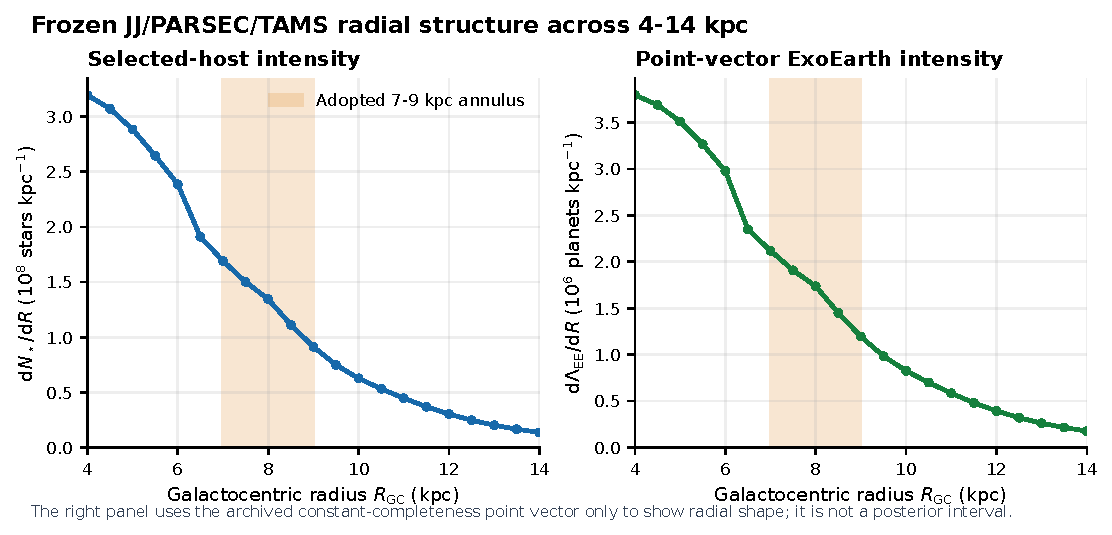
\includegraphics[width=0.96\textwidth]{v4_radial_annulus.pdf}
\caption{Frozen radial structure of the selected JJ/PARSEC/TAMS host population
across 4--14 kpc. The adopted 7--9 kpc annulus is shaded. The right panel
applies the archived constant-completeness point vector only to expose the
radial shape of the propagated estimator; it is not a posterior interval and
does not replace the posterior summaries in Section~\ref{sec:results}.}
\label{fig:radial}
\end{figure*}

\section{Occurrence Posterior and Habitable-Zone Integration}\label{sec:occurrence}

\subsection{Bryson occurrence function}

We adopt Model~1 from \citet{Bryson2021}. The differential number of planets
per star per unit $r$ and $I$ is
\begin{equation}
 \lambda(r,I,T\mid\bm\theta)
 =F_0C_1r^\alpha I^\beta T^\gamma g(T),
 \label{eq:lambda}
\end{equation}
where $\bm\theta=(F_0,\alpha,\beta,\gamma)$ is written in manuscript order,
$T$ is in kelvin, and
\begin{equation}
 g(T)=
 \begin{cases}
 10^{-11.839}T^{3.16}, & T\leq5117\ {\rm K},\\
 10^{-16.769}T^{4.49}, & T>5117\ {\rm K}.
 \end{cases}
 \label{eq:gT}
\end{equation}
$C_1$ normalizes the model over $0.5\leq r\leq2.5$,
$0.2\leq I\leq2.2$, and a uniform temperature measure over 3900--6300 K.
Appendix~\ref{app:analytic} gives the analytic normalization.

The constant- and zero-completeness treatments are distinct likelihood
scenarios inherited from the source analysis. They are not samples from one
mixture distribution and are not assigned model probabilities here. The
source interpretation places the unknown long-period completeness between
these cases, but this statement is conditional on the adopted extrapolation
family rather than an assumption-free physical bound.

\subsection{Corrected catalog-error propagation}\label{subsec:measurement}

For a catalog value $\mu$ with reported lower and upper uncertainties
$\sigma_-$ and $\sigma_+$, the v4 primary analysis draws
\begin{align}
 B&\sim{\rm Bernoulli}(1/2),\qquad U=|Z|,\quad Z\sim\mathcal{N}(0,1),\nonumber\\
 X&=\begin{cases}
 \mu-\sigma_-U,&B=0,\\
 \mu+\sigma_+U,&B=1.
 \end{cases}
 \label{eq:measurement_draw}
\end{align}
This construction places the quoted one-sigma lower and upper excursions at
the 15.9th and 84.1st percentiles when the uncertainties are interpreted as
two-sided Gaussian-equivalent errors. It replaces the source notebook's
signed-normal mixture, which does not preserve the intended association
between direction and asymmetric scale. After perturbing instellation, radius,
and $\Teff$, all source-domain conditions are reapplied:
\begin{equation}
 0.2\leq I\leq2.2,
 \quad0.5\leq r\leq2.5,
 \quad3900\leq T\leq6300\ {\rm K}.
 \label{eq:source_domain}
\end{equation}
The source-faithful legacy mechanism is retained only as a regression and
sensitivity mode.

Each outer realization also applies the catalog reliability mechanism before
fitting. Thus the calculation marginalizes over the implemented reliability
and measurement procedure, but not over unmodeled catalog systematics or
occurrence functional forms.

\subsection{Poisson likelihood and adaptive MCMC}\label{subsec:mcmc}

For retained candidates $x_p=(I_p,r_p,T_p)$, the source inhomogeneous-Poisson
log likelihood can be written schematically as
\begin{equation}
 \log\mathcal{L}(\bm\theta)
 =\sum_p\log\lambda(x_p\mid\bm\theta)
 -\int\lambda(x\mid\bm\theta)C(x)\,\dd x,
 \label{eq:poisson_likelihood}
\end{equation}
where $C(x)$ is the branch-specific summed completeness surface evaluated on
the source grid. We retain the source uniform priors inside its numerical
bounds: $0\leq F_0<50000$, $-5\leq\alpha<5$,
$-5\leq\beta<5$, and $-500\leq\gamma<50$, with zero density outside.

For each completeness branch we generate 400 independently seeded outer
reliability/measurement realizations. Each four-parameter conditional
posterior is sampled with 16 ensemble walkers after 1000 discarded burn-in
steps. Autocorrelation time is checked every 1000 production steps. Acceptance
requires, for every parameter, at least $100\tau$, no more than 5\% relative
change between successive $\tau$ estimates, and two consecutive qualifying
checks. The constant production used a 20,000-step ceiling. Five zero-branch
realizations reached that ceiling without satisfying the unchanged gate, so
the entire zero branch was rerun with identical seeds and criteria and a
30,000-step ceiling; no failed realization was discarded.

Adaptive chains have unequal lengths. The aggregation therefore retains 1024
deterministically spaced post-burn rows from every outer realization, assigning
equal weight to each catalog realization. Outer quantile Monte Carlo error is
estimated by resampling whole realizations as clusters; matched contiguous
chain blocks diagnose residual inner-chain error. The two completeness
branches remain separate through this aggregation and the Galactic propagation.

\subsection{Present-day conservative HZ}

For a climatic boundary, the effective stellar flux is
\begin{align}
 S_{\rm eff}(T)={}&S_{{\rm eff},\odot}+aT'
 +bT'^2+cT'^3+dT'^4,\nonumber\\
 T'={}&T-5780\ {\rm K},
 \label{eq:kopparapu}
\end{align}
using the corrected coefficients of \citet{Kopparapu2013,Kopparapu2013Erratum}. The canonical conservative HZ uses the
$1\,\Mearth$ runaway-greenhouse inner boundary from \citet{Kopparapu2014} and
the maximum-greenhouse outer boundary. ``Conservative'' names this prescribed
boundary pair; it is not a universal lower bound over climate models.

Let $S_{\rm out}(T)$ and $S_{\rm in}(T)$ denote the outer and inner flux
boundaries. The broad HZ and narrow target domains are
\begin{equation}
 \mathcal{D}_{\rm HZ}(T)
 =[0.5,1.5]\times[S_{\rm out}(T),S_{\rm in}(T)],
 \label{eq:d_hz}
\end{equation}
\begin{align}
 \mathcal{D}_{\rm EE}(T)=[0.9,1.1]\times
 \big[&\max\{0.9,S_{\rm out}(T)\},\nonumber\\
      &\min\{1.1,S_{\rm in}(T)\}\big],
 \label{eq:d_ee}
\end{align}
with an empty domain when the upper limit does not exceed the lower. Across
5300--6000 K the outer HZ does not clip $I=0.9$; the runaway-greenhouse
boundary crosses $I=1.1$ at 5727.1 K and clips the inner edge at lower
temperatures.

\begin{figure*}[t]
\centering
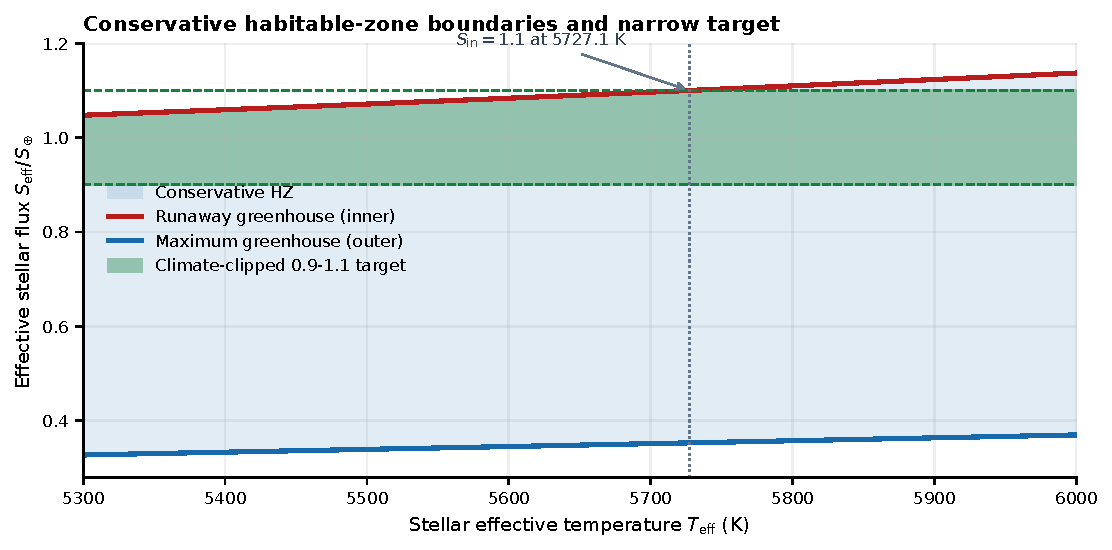
\includegraphics[width=0.96\textwidth]{v4_hz_boundaries.pdf}
\caption{Conservative habitable-zone boundaries over the selected stellar
temperature range. The broad shaded region lies between the
maximum-greenhouse and $1\,\Mearth$ runaway-greenhouse flux limits. The darker
region is the resulting climate-clipped intersection with the fixed
$0.9\leq I\leq1.1$ narrow target; its hot-side behavior changes where the
runaway boundary crosses $I=1.1$.}
\label{fig:hzboundaries}
\end{figure*}

\subsection{Posterior Galactic estimator}

For $k\in\{{\rm HZ},{\rm EE}\}$ and posterior draw $s$, the expected planets
per star at temperature $T$ are
\begin{equation}
 f_{k,s}(T)=\iint_{\mathcal{D}_k(T)}
 \lambda(r,I,T\mid\bm\theta_s)\,\dd r\,\dd I.
 \label{eq:fk}
\end{equation}
At radial node $R_j$, the occurrence-weighted surface density is
\begin{equation}
 \Sigma_{k,s}(R_j)=\sum_i H_{ij}w_{ij}f_{k,s}(T_{ij}).
 \label{eq:sigma_k}
\end{equation}
The propagated estimator is
\begin{equation}
 \boxed{
 \Lambda_{k,s}^{(\Delta R)}
 =10^6\Delta R\sum_{j=0}^{4}c_j\,2\pi R_j
 \sum_i H_{ij}w_{ij}f_{k,s}(T_{ij}) .}
 \label{eq:galactic_estimator}
\end{equation}
Posterior summaries are quantiles of $\{\Lambda_{k,s}\}$ after equalizing the
outer-realization mixture. Equation~(\ref{eq:galactic_estimator}) preserves the
temperature dependence of both occurrence and HZ clipping; it is not a single
rate multiplied by a host count.

\begin{figure*}[t]
\centering
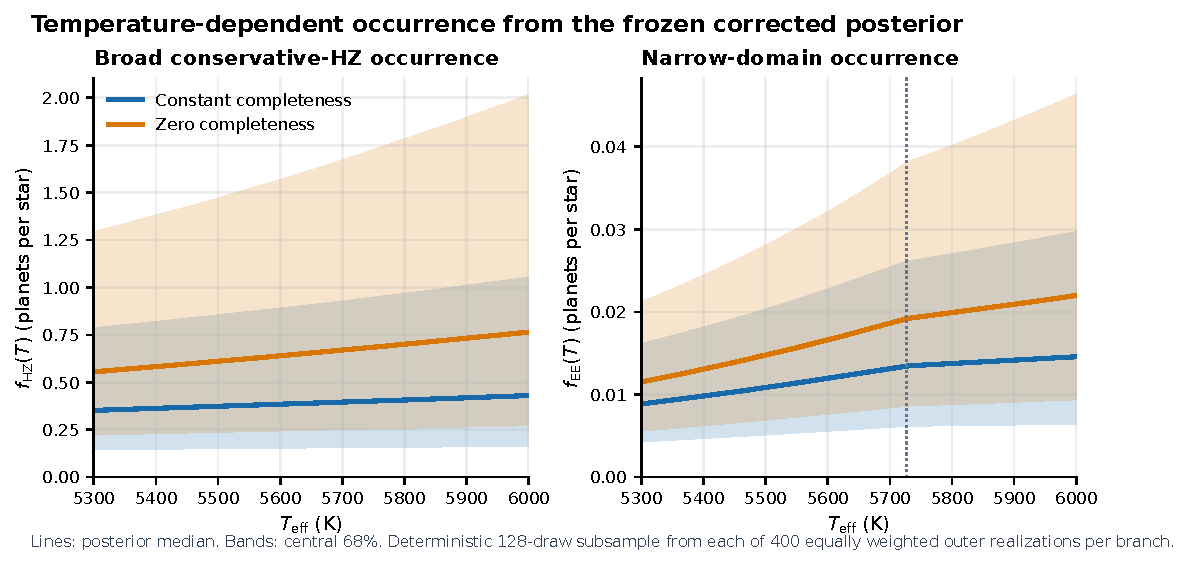
\includegraphics[width=0.96\textwidth]{v4_occurrence_vs_teff.pdf}
\caption{Temperature-dependent broad-HZ and narrow-target occurrence implied
by the frozen corrected posterior. Lines are posterior medians and shaded
bands are central 68\% intervals. For plotting only, each branch uses a
deterministic 128-draw subsample from every one of its 400 equally weighted
outer realizations (51,200 draws per branch); the numerical tables and
headline posterior summaries remain those of the full frozen propagation.}
\label{fig:occurrence-teff}
\end{figure*}

\section{Results}\label{sec:results}

\subsection{Host population}

The canonical selector yields
\begin{equation}
 N_\star=263{,}061{,}992.37
 \label{eq:nstar_result}
\end{equation}
model hosts in the 7--9 kpc annulus. The thin disk contributes
$2.11\times10^8$ and the thick disk $5.23\times10^7$, or 19.9\% of the total.
From the pre-TAMS parent measure of $2.9877\times10^8$, the radius boundary
rejects $3.3857\times10^7$ and the compact-object veto rejects
$1.8513\times10^6$ in the mutually exclusive audit decomposition.
Table~\ref{tab:demographics} summarizes the selected host distribution.

\begin{table*}[t]
\caption{Integrated host-property distribution in the 7--9 kpc annulus}
\label{tab:demographics}
\centering
\begin{tabular}{lccrrrr}
\toprule
Quantity & Unit & Weighted mean & 16th percentile & Median & 84th percentile\\
\midrule
Effective temperature & K & 5646 & 5424 & 5670 & 5841\\
Age & Gyr & 9.35 & 6.41 & 9.59 & 12.16\\
$[\mathrm{Fe/H}]$ & dex & -0.020 & -0.284 & +0.033 & +0.222\\
Current mass & $M_\odot$ & 0.913 & 0.810 & 0.910 & 1.015\\
Stellar radius & $R_\odot$ & 1.035 & 0.864 & 0.999 & 1.237\\
$\log g$ & dex (cgs) & 4.379 & 4.250 & 4.400 & 4.492\\
\bottomrule
\end{tabular}
\end{table*}

The genuine solar-composition low-mass phase-7 curve selects exactly the same
integrated population as the inherited one-dimensional boundary. In
particular, omitting the special 5200 K table anchor changes $N_\star$ and the
plug-in $\LamEE$ by 0.0000\%. This validates the numerical implementation but
does not quantify uncertainty from metallicity, helium abundance, or
isochrone-family choice.

\subsection{Occurrence and Galactic expectations}

Table~\ref{tab:posterior_results} gives the frozen posterior quantiles. Under
constant completeness, the median narrow-domain occurrence is 0.01226 planets
per selected star and the propagated median is
\begin{equation}
 \LamEE^{\rm const}=3.224\times10^6,
 \quad 68\%:\ [1.522,6.189]\times10^6.
 \label{eq:canonical_results}
\end{equation}
Under zero completeness,
\begin{equation}
 \LamEE^{\rm zero}=4.572\times10^6,
 \quad 68\%:\ [2.103,8.912]\times10^6.
 \label{eq:zero_results}
\end{equation}
The corresponding 95\% intervals are $0.652$--$10.842$ million and
$0.888$--$15.840$ million. The branch medians differ by 41.83\%, but that
difference is a model scenario contrast rather than a credible-interval
component.

\begin{table*}[t]
\caption{Frozen posterior occurrence and Galactic population quantiles}
\label{tab:posterior_results}
\centering
\small
\setlength{\tabcolsep}{5pt}
\begin{tabular}{llrrrrr}
\toprule
Branch & Quantity & 2.5\% & 16\% & Median & 84\% & 97.5\%\\
\midrule
Constant & $\langle\fHZ\rangle$ & 0.0645 & 0.1601 & 0.3883 & 0.9070 & 1.9967\\
Constant & $\langle\fEE\rangle$ & 0.00248 & 0.00579 & 0.01226 & 0.02353 & 0.04121\\
Constant & $\LamHZ$ ($10^6$) & 16.971 & 42.104 & 102.148 & 238.593 & 525.246\\
Constant & $\LamEE$ ($10^6$) & 0.652 & 1.522 & 3.224 & 6.189 & 10.842\\
\midrule
Zero & $\langle\fHZ\rangle$ & 0.0965 & 0.2537 & 0.6591 & 1.6216 & 3.7502\\
Zero & $\langle\fEE\rangle$ & 0.00338 & 0.00799 & 0.01738 & 0.03388 & 0.06021\\
Zero & $\LamHZ$ ($10^6$) & 25.394 & 66.746 & 173.376 & 426.579 & 986.540\\
Zero & $\LamEE$ ($10^6$) & 0.888 & 2.103 & 4.572 & 8.912 & 15.840\\
\bottomrule
\end{tabular}
\tablecomments{Occurrence quantities are planets per star, not fractions of
stars. Intervals are conditional on the fitted Model~1 occurrence surface and
the frozen host/HZ construction.}
\end{table*}

Within matched posterior draws, the narrow target contains a median 3.119\%
of broad-HZ occurrence in the constant branch and 2.606\% in the zero branch.
This ratio is derived from the same occurrence model; it is not an independent
planet fraction.

\begin{figure*}[t]
\centering
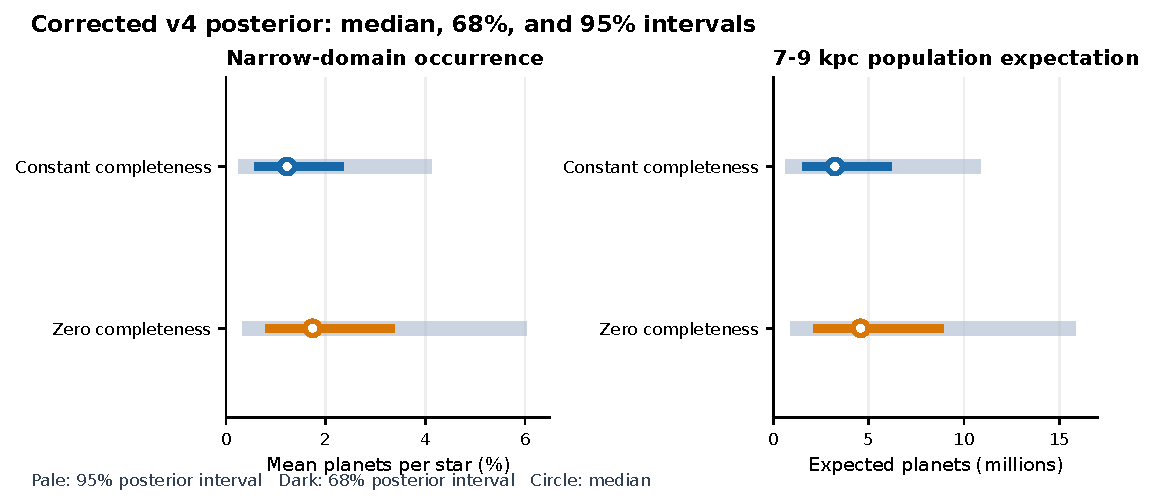
\includegraphics[width=0.96\textwidth]{v4_posterior_intervals.pdf}
\caption{Corrected posterior summaries for narrow-domain occurrence, expressed
as expected planets per 100 stars rather than a percentage of planet-hosting
stars (left), and the propagated 7--9 kpc population expectation (right). Pale and
dark segments show 95\% and 68\% posterior intervals; circles mark medians.
The two completeness branches are separate scenarios. These intervals do not
include occurrence-model-form, local-support, host-population, climate, or
transport uncertainty.}
\label{fig:posterior}
\end{figure*}

\section{Verification and Empirical-Support Audit}\label{sec:verification}

\subsection{Statistical and numerical gates}

All 400 constant-branch and all 400 zero-branch outer realizations passed the
adaptive convergence gate. The minimum, median, and maximum production lengths
were 8000, 12,000, and 17,000 steps for the constant branch and 9000, 14,000,
and 22,000 for the zero branch. The minimum effective sample size over every
parameter and realization was 1682.3 and 1662.4, respectively. There were no
optimizer failures.

The largest outer-realization median Monte Carlo standard error, expressed as
a fraction of the associated 16th--84th percentile width, was 1.63\% for the
constant branch and 1.56\% for zero completeness. The corresponding maximum
inner-chain fractions were 0.10\% and 0.15\%. Independent MCMC-seed families
passed the frozen stability comparison. These values are far below the
predeclared 10\% outer and 5\% inner gates.

The measurement implementation has a bitwise source-faithful legacy regression
mode and a corrected quantile-recovery suite. Aggregation rejects mixed modes,
unequal outer weights, failed convergence, and inconsistent diagnostic
metadata. The host/HZ propagation separately verifies non-negative weights,
nested domains, unit conversions, and reproduction of the frozen quantiles.
Refining the radial grid from 0.5 to 0.25 kpc changes the plug-in $\LamEE$ by
+0.231\%, below the predeclared 1\% numerical threshold.

These checks establish engineering and numerical consistency of the frozen
pipeline. They do not establish that the separable occurrence surface is an
adequate scientific description inside the target box.

\subsection{Direct DR25 support}\label{subsec:dr25support}

The exact target is geometrically contained in the fitted DR25 source domain:
$0.9$--$1.1\,\Rearth$ lies inside $0.5$--$2.5\,\Rearth$,
$0.9$--$1.1\,\Searth$ lies inside $0.2$--$2.2\,\Searth$, and the selected
temperatures lie inside 3900--6300 K. Geometric containment, however, does not
guarantee local data support.

The merged nominal planet-candidate catalog contains 2277 rows. Fifty-four
rows lie in the fitted source domain after the nominal cuts, with summed total
reliability 42.23. For the selected 5300--6000 K stars, 54 candidates satisfy
the narrow radius range, while only three satisfy the conservative-HZ
instellation intersection. No nominal candidate satisfies the radius and
fixed 0.9--1.1 instellation box simultaneously; the exact climate-clipped
target therefore has candidate count zero and reliability sum zero.

Across 400 corrected outer realizations, the constant branch has target-count
quantiles $(0,0,0,0,1)$ at probabilities $(2.5,16,50,84,97.5)$\% and a
95.75\% zero-count fraction. The zero branch has the same quantile vector and
a 96.75\% zero-count fraction. Only K08107.01 and K08242.01 enter the target
under any perturbation, with 17 total appearances in the constant branch and
13 in the zero branch. Consequently, the local empirical-support gate is a
scientific \emph{failure}, even though the geometry and code checks pass.

\begin{figure*}[t]
\centering
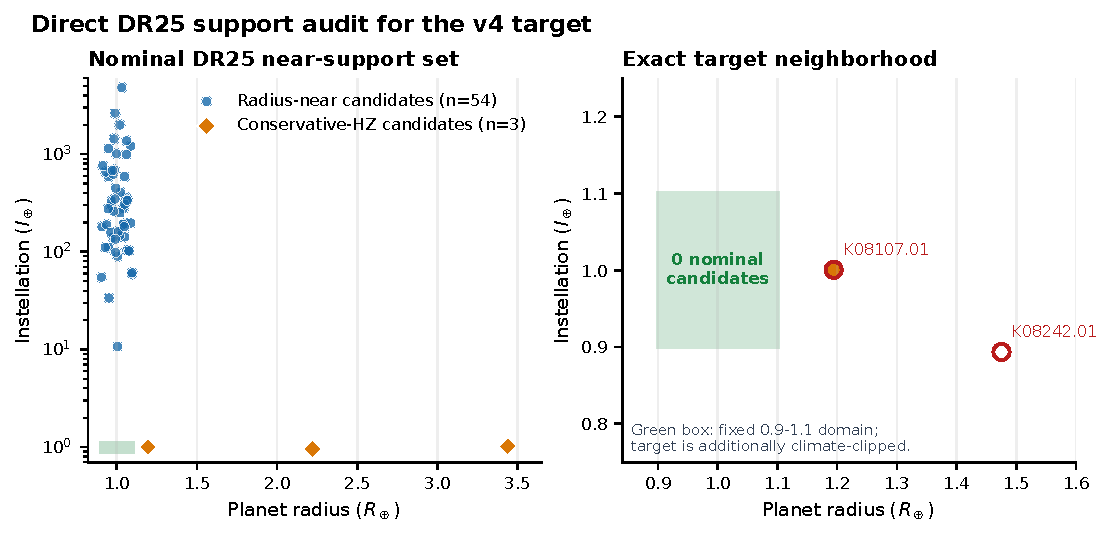
\includegraphics[width=0.96\textwidth]{v4_dr25_local_support.pdf}
\caption{Nominal DR25 candidates near one component of the target selection.
Left: radius-near and conservative-HZ-near candidates for 5300--6000 K hosts;
the fixed target box is green. Right: the exact neighborhood, with the two
nominal candidates that can enter only after measurement perturbation outlined
in red. The climate condition further clips the fixed green box. No nominal
candidate lies in the full target.}
\label{fig:dr25support}
\end{figure*}

\section{Source-Model Fidelity Benchmark}\label{sec:benchmark}

\citet{Bryson2021} report broad conservative-HZ occurrence of 0.37 planets per
star under high completeness and 0.60 under low completeness for their broader
$0.5$--$1.5\,\Rearth$, 4800--6300 K definition. The reconstructed v4 broad-HZ
medians are 0.388 and 0.659. The agreement in scale supports source fidelity,
but it is not independent validation: the present posterior is reconstructed
from the same public DR25 model and inputs.

The point-vector reference inherited from version~3 gives
$\LamEE=3.3765\times10^6$ for the constant branch. The corrected posterior
median is $3.2238\times10^6$; these are different statistical functionals and
need not coincide. The v4 inference uses the pooled equal-weight joint
posterior rather than independently sampled marginal summaries or a scaled
broad-HZ interval.

\section{Sensitivity and Uncertainty}\label{sec:sensitivity}

The frozen register separates posterior scenarios, numerical checks, model
alternatives, climate prescriptions, alternative estimands, categorical
validation failures, and unparameterized systematics. These entries are not
exchangeable random errors and are not combined in quadrature.

\begin{table*}[t]
\caption{Audited sensitivity of the narrow ExoEarth expectation}
\label{tab:sensitivity}
\centering
\small
\begin{tabular}{llrl}
\toprule
Category & Comparison & Change in $\LamEE$ & Statistical role\\
\midrule
Measurement & Legacy versus corrected propagation & +0.026\% & Posterior q50 regression\\
Completeness & Zero versus constant branch & +41.83\% & Separate scenario\\
Host selector & Legacy fixed-$\log g$, constant & -28.58\% & Posterior model sensitivity\\
Host selector & Legacy fixed-$\log g$, zero & -29.58\% & Posterior model sensitivity\\
TAMS & Native curve without 5200 K anchor & 0.000\% & Plug-in numerical validation\\
Numerics & Radial grid 0.5 to 0.25 kpc & +0.231\% & Plug-in convergence check\\
Occurrence & Bryson Model~2 versus Model~1 & +3.30\% & Point-vector model alternative\\
Climate & Inner HZ flux $\times0.95$ & -24.84\% & Boundary perturbation\\
Climate & Inner HZ flux $\times1.05$ & +7.15\% & Boundary perturbation\\
Climate & $0.1\,\Mearth$ runaway boundary & -57.28\% & Alternative prescription\\
Climate & $5\,\Mearth$ runaway boundary & +7.15\% & Alternative prescription\\
HZ definition & Optimistic versus conservative & +7.15\% & Alternative estimand\\
Temperature & JJ weighted versus uniform & +0.380\% & Weighting diagnostic\\
\bottomrule
\end{tabular}
\tablecomments{The basis differs by row and is stated explicitly. Posterior
rows use branch-specific medians; point-vector rows use the frozen constant
reference $3.3765\times10^6$. None is an added posterior error bar.}
\end{table*}

The legacy measurement algorithm changes the constant posterior median by only
0.026\%, so correcting its asymmetric-error construction is methodologically
necessary but does not drive the headline median. The host selector and climate
prescription have much larger effects. Model~2 changes the point estimate by
3.30\%, but no Model~2 posterior was propagated and that single alternative
does not span arbitrary radius--instellation structure.

The $\pm1\%$ inner-boundary perturbations are asymmetric: multiplying the
runaway-greenhouse flux by 0.99 changes the plug-in result by -3.67\%, whereas
a factor 1.01 gives +2.71\%. Factors 0.95 and 1.05 give -24.84\% and +7.15\%.
This nonlinearity follows from clipping the fixed 0.9--1.1 instellation box by
the temperature-dependent inner HZ. The $0.1$ and $5\,\Mearth$ rows alter the
published climate prescription; they do not model the unknown planet-mass
distribution inside the radius interval.

\begin{figure*}[t]
\centering
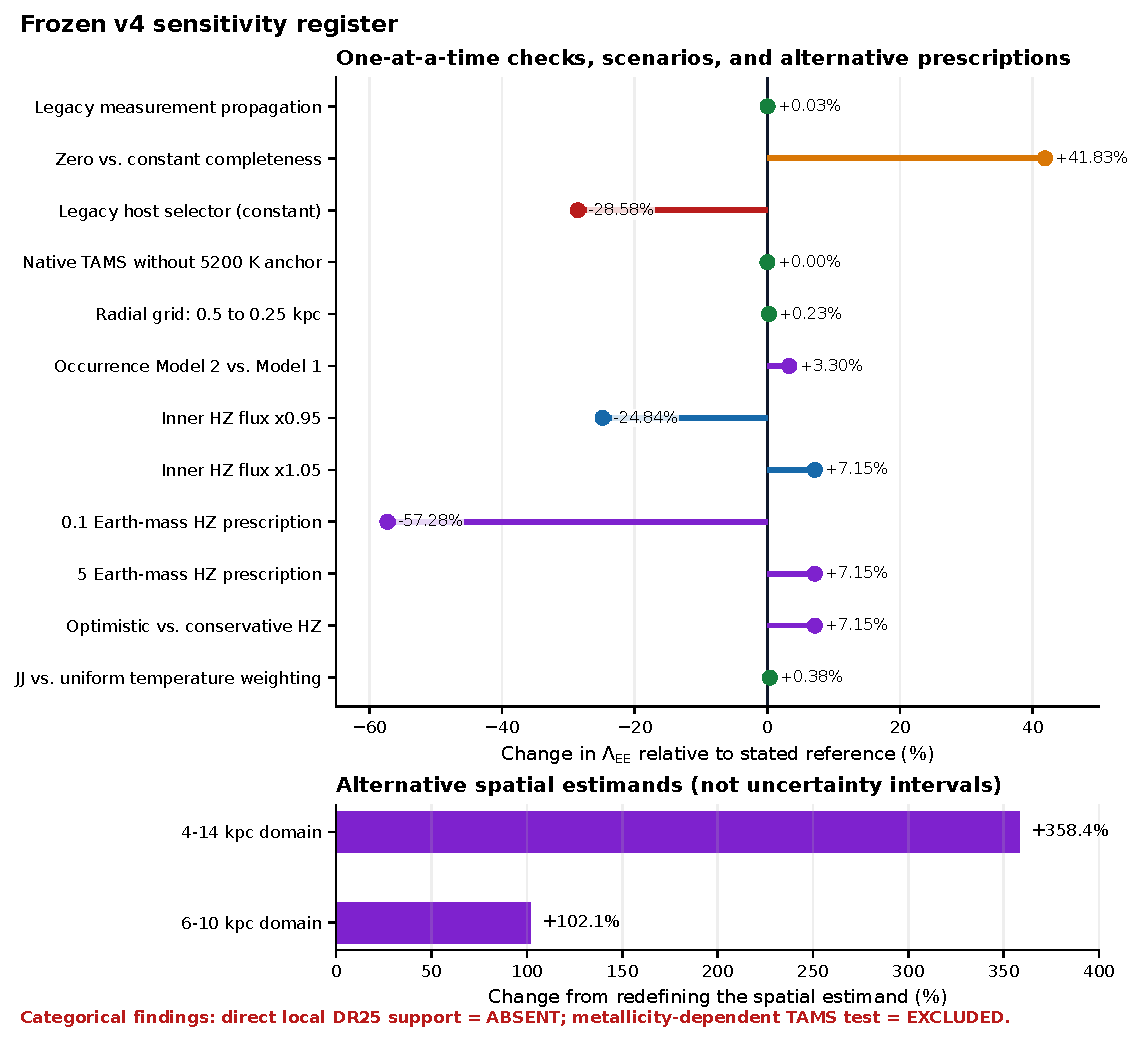
\includegraphics[width=0.95\textwidth]{v4_sensitivity_register.pdf}
\caption{Frozen one-at-a-time sensitivity register. Colors distinguish
numerical checks, scenarios, model alternatives, and alternative prescriptions.
Spatial-domain changes are shown separately because they redefine the target
population. The DR25 local-support failure and excluded metallicity-TAMS test
are categorical findings, not plotted numerical error bars.}
\label{fig:sensitivity}
\end{figure*}

Changing the radial mask changes the estimand. Relative to the 7--9 kpc
constant point-vector result, the 6--10 kpc domain gives
$\LamEE=6.8239\times10^6$ (+102.10\%) and the full 4--14 kpc JJ domain gives
$1.5479\times10^7$ (+358.43\%). They are alternative populations rather than
uncertainty intervals for the annulus.

The archived metallicity-dependent TAMS surface is not a valid sensitivity.
Its input contains 42 giant or high-mass phase-7 contaminants, reaching
$155\,M_\odot$ and $2312\,R_\odot$, while several low-metallicity tracks do not
cover 5300--6000 K. The previously reported +1.59\% change is retracted and
excluded. A valid low-mass metallicity-dependent TAMS analysis remains open.

Other unparameterized epistemic uncertainties remain open: JJ component
normalization and star-formation history, isochrone family, radial migration,
multiplicity mismatch, occurrence transport with age and metallicity, and
occurrence functional form in the locally empty target. No defensible joint
distribution is available, so a combined total uncertainty is not reported.

\section{Discussion}\label{sec:discussion}

\subsection{Comparison with primary occurrence studies}

Published Earth-analog occurrence estimates are not interchangeable because
their radius, orbital coordinate, HZ definition, stellar sample, catalog, and
reported statistical functional differ. The v4 median occurrence is 0.0123
and 0.0174 planets per star under constant and zero completeness, respectively
(equivalently, 1.23 and 1.74 expected planets per 100 stars, not percentages of
stars hosting planets). These values are numerically below broad-HZ estimates
as expected for the much narrower integrated phase space.

\citet{Bryson2021} use $0.5$--$1.5\,\Rearth$ and a complete conservative HZ.
Their temperature-matched 5300--6000 K G-star values of 0.38 and 0.63 are the
primary source-fidelity anchors for this analysis; the broader 4800--6300 K
$\eta_\oplus$ values of 0.37 and 0.60 provide wider context. Neither comparison
is independent corroboration. \citet{Kunimoto2020} report an 84.1\% upper limit below 0.18
planets per G star for $0.75$--$1.5\,\Rearth$ and 0.99--1.70 au; semimajor axis,
radius, and host definitions all differ from v4. The conceptually narrower
$\zeta_{1.0}$ of \citet{Burke2015} uses planet radius and orbital period within
20\% of Earth, yielding a central value near 0.1 but an allowed 0.01--2 range
once major statistical and systematic uncertainty is considered.

Using a stripped-core-aware occurrence interpretation, \citet{Pascucci2019}
obtain broad-HZ values of roughly 5--10\% and show that extrapolation choices
can change the result by factors of several. \citet{Bergsten2022} report
$\Gamma_\oplus=15^{+6}_{-4}\%$, a local differential density per logarithmic
period--radius area rather than an integrated planets-per-star quantity for the
v4 box. Converting it would require an explicit domain and occurrence model.

No one of these primary results simultaneously matches the v4 radius,
instellation, climate intersection, host-temperature range, and catalog/model
definition. Point-estimate differences therefore do not by themselves
establish inconsistency. The common conclusion relevant here is that sparse
long-period data and occurrence-model form are material epistemic limitations.

\subsection{Local support and model-form risk}

The zero-candidate audit sharpens the limitation that version~3 described only
as sparsity. The posterior remains mathematically finite because a separable
power law is fitted over the larger source domain and then integrated over the
target. Thus the interval describes uncertainty in that fitted projection; it
does not demonstrate that the local surface is smooth, separable, or free of a
break near Earth radius and instellation.

The Model~2 point comparison is useful but insufficient. It changes one
temperature parameterization within the Bryson framework and does not test
arbitrary curvature, radius--instellation interactions, or stripped-core
structure \citep{LopezRice2018,Pascucci2019}. A more complete analysis would
fit competing occurrence surfaces to the same perturbed catalogs and perform
posterior predictive checks targeted at the empty local region.

\subsection{Host-population and transport uncertainty}\label{subsec:transport}

The JJ host count is a deterministic output of the pinned parameter realization
and isochrone library. The sub-percent radial-grid change is only a numerical
diagnostic. Posterior uncertainty in star-formation and age--metallicity
histories, IMF parameters, component normalizations, radial migration, and the
choice among PARSEC, MIST, and BaSTI is not propagated. The reported host count
is reproducible but not astrophysically known to sub-percent precision.

Equation~(\ref{eq:galactic_estimator}) transports a Kepler-calibrated model to
an older Galactic population. Conditional on $\Teff$, it assumes no additional
dependence of planet occurrence or survival on age, $[\mathrm{Fe/H}]$,
$[\alpha/\mathrm{Fe}]$, disk membership, or Galactocentric radius. This is a
null transport assumption, not an empirical result.

Current empirical evidence does not justify replacing that null with one
universal correction. For close-in planets, \citet{Dai2021} find lower
$1$--$4\,\Rearth$, $P<100$ day occurrence around high-velocity stars, but the
reported separation depends on how correlated stellar properties are
controlled. \citet{BashiZucker2022} likewise find more close-in super-Earths
around their younger, slower, metal-richer thin-disk sample than around the
older thick-disk sample, while emphasizing the small thick-disk and halo
planet samples and the covariance among age, chemistry, and kinematics. In
contrast, the direct DR25 age-binned analysis of \citet{Sayeed2025} finds no
statistically significant overall occurrence--age trend for FGK stars; only a
weak decrease appears in the low-mass, metal-rich subset. These studies probe
shorter periods and much broader radius domains than the present HZ target.
Together they foreground an unresolved transport uncertainty, not a measured
multiplicative adjustment to Equation~(\ref{eq:galactic_estimator}).

The Kepler source denominator also includes observational-quality and binary
cuts that the intrinsic JJ single-star population does not reproduce. Close
companions can suppress planet occurrence \citep{Kraus2016}, while unresolved
multiplicity alters radii and completeness. The direction and magnitude of a
correction cannot be identified from the current inputs, so multiplicity
remains unquantified rather than receiving an ad hoc factor.

\subsection{Meaning of the Galactic annulus}

The 7--9 kpc interval is an absolute geometric mask motivated by historically
highlighted Galactic-habitable-zone work \citep{Lineweaver2004}; it does not
import that study's time-dependent metallicity, supernova, terrestrial-planet,
or biological weighting. Sharply bounded Galactic habitable zones are
themselves model-dependent \citep{Prantzos2008,Gowanlock2011}. The present
result is therefore an estimate within an annulus, not the number of ExoEarth
candidates in a physically complete Galactic habitable zone.

The annulus also describes present-day position rather than formation
environment. Using an action-, age-, and chemistry-based model of APOGEE
low-$\alpha$ disk stars, \citet{Frankel2020} find that angular-momentum
redistribution is substantially stronger than radial heating. Hence a star now
inside 7--9 kpc need not have formed there, and a star born there need not
remain there. Because the present calculation does not model birth radii or
planet survival along migrated orbits, it must not be interpreted as a sharply
bounded birth-annulus census.

\subsection{What the reported values mean}

The statement $\LamEE=3.22$ million in the constant branch means that the
frozen model stack assigns that median expected number of planets to the stated
radius--instellation--present-day-HZ domain and host population. The zero branch
assigns 4.57 million under a different completeness extrapolation. These are
not observed counts, not numbers of systems with at least one selected planet,
and not counts of rocky, ocean-bearing, habitable, or inhabited worlds.

The displayed posterior intervals are statistically meaningful for the
implemented conditional model, but narrower in scope than the total scientific
uncertainty. Reproducibility of a conditional projection and empirical validity
of the projection are separate questions; v4 passes the former and explicitly
fails the local-support component of the latter.

\section{Conclusions}\label{sec:conclusions}

We reconstructed and propagated a corrected joint occurrence posterior through
a temperature-resolved Galactic host measure. For the specified old G-star
population in the 7--9 kpc annulus, the frozen host model gives
$N_\star=2.6306\times10^8$. The narrow-domain posterior results are
\begin{align}
 \LamEE^{\rm const}&=3.22^{+2.97}_{-1.70}\ {\rm million},\nonumber\\
 \LamEE^{\rm zero}&=4.57^{+4.34}_{-2.47}\ {\rm million},
\end{align}
where uncertainties are 16th--84th percentile posterior intervals within each
separate completeness scenario.

All 800 outer MCMC realizations pass the adaptive convergence gate, the outer
and inner quantile Monte Carlo errors are small relative to posterior width,
the radial quadrature is stable below 0.3\%, and the native low-mass solar TAMS
curve reproduces the canonical host selection. The legacy measurement mechanism
changes the constant median by only 0.026\%.

The main scientific limitation is not numerical. There are zero nominal DR25
candidates and zero summed reliability in the exact target, and more than 95\%
of corrected catalog realizations also contain zero. Occurrence-model form,
host normalization, climate prescription, stellar multiplicity, and Galactic
transport are not contained in the posterior intervals. The defensible
conclusion is therefore conditional: the fitted separable Bryson Model~1
surface, transported through the frozen JJ/PARSEC/TAMS population, projects a
median of several million narrow-domain candidates into this annulus. The work
does not provide a direct candidate-supported measurement or a complete
astrophysical uncertainty budget.

\section{Data and Software Availability}\label{sec:data}

The public project repository is
\url{https://github.com/jerseroman/are-we-alone-in-the-universe}.
The persistent project concept DOI is
\href{https://doi.org/10.5281/zenodo.20474527}{10.5281/zenodo.20474527}; exact
reproduction additionally requires the v4 release record and commit identified
in its checksum manifest.

The immutable manuscript-v3 source is commit
\hashid{5a3528aea6d6f28da8e9db4d40f0c84cbb43d501}. The v4 source-provenance
manifest records the source tree and every imported LaTeX/BibTeX blob before
editing. The Bryson research-code source is
\hashid{d200f54b6f0df49e0dae530e69983cdce5397bfb}. Corrected-posterior execution
is recorded by GitHub Actions runs 32470830404, 32472776218, 32506666772, and
32527877921. The release evidence contains the frozen numerical, host/TAMS,
DR25-support, sensitivity, and primary-literature records together with
SHA-256 manifests.

The analysis uses Python, NumPy \citep{Harris2020}, pandas
\citep{McKinney2010}, Matplotlib \citep{Hunter2007}, Astropy
\citep{Astropy2022}, \texttt{emcee} \citep{ForemanMackey2013}, and
\texttt{jjmodel} \citep{Sysoliatina2022}. The manuscript figures are generated
only from committed frozen CSV/JSON artifacts. Local raw production artifacts
are represented by their recorded hashes and GitHub Actions run identifiers;
the reproducibility archive supplies the compact frozen outputs required to
audit every reported number.

\appendix
\setcounter{equation}{0}
\renewcommand{\theequation}{A\arabic{equation}}
\renewcommand{\theHequation}{A.\arabic{equation}}

\section{Analytic Occurrence Integrals}\label{app:analytic}

For exponent $q$, define
\begin{equation}
 \mathcal{J}(x_0,x_1;q)=
 \begin{cases}
 \displaystyle\frac{x_1^{q+1}-x_0^{q+1}}{q+1}, & q\neq-1,\\[6pt]
 \ln(x_1/x_0), & q=-1.
 \end{cases}
 \label{eq:primitive}
\end{equation}
With $T_0=3900$ K, $T_b=5117$ K, and $T_1=6300$ K, the Model~1 normalization is
\begin{align}
 C_1^{-1}={}&
 \mathcal{J}(0.5,2.5;\alpha)
 \mathcal{J}(0.2,2.2;\beta)\nonumber\\
 &\times\frac{1}{T_1-T_0}\big[
 10^{-11.839}\mathcal{J}(T_0,T_b;\gamma+3.16)\nonumber\\
 &\hspace{36mm}+10^{-16.769}\mathcal{J}(T_b,T_1;\gamma+4.49)
 \big].
 \label{eq:c1}
\end{align}
Because Equation~(\ref{eq:lambda}) is separable within each temperature branch, $f_k(T)$ is evaluated analytically in $r$ and $I$ using Equation~(\ref{eq:primitive}). The only numerical quadrature in the final Galactic estimator is the radial integration after the row-level sums have been constructed.

\section{Bryson Model~2 Sensitivity}\label{app:model2}

For the Model~2 sensitivity, the source occurrence function is
\begin{equation}
 \lambda_2(r,I,T\mid\bm\theta_2)=F_0C_2r^\alpha I^\beta T^\gamma,
 \label{eq:model2}
\end{equation}
without the fixed geometric factor $g(T)$. Its normalization is
\begin{equation}
 C_2^{-1}=\mathcal{J}(0.5,2.5;\alpha)
 \mathcal{J}(0.2,2.2;\beta)
 \frac{\mathcal{J}(T_0,T_1;\gamma)}{T_1-T_0}.
 \label{eq:c2}
\end{equation}
The adopted \citet{Bryson2021} \texttt{hab2}, Poisson, ``With Uncertainty,'' constant-completeness median vector is
\begin{equation}
 (F_0,\alpha,\beta,\gamma,C_2)
 =(1.13,-1.13,-0.85,+1.19,1.072724\times10^{-5}).
\end{equation}
Evaluated on the same frozen JJ rows and HZ prescription, this gives $\LamEE=3.487759\times10^6$, or $+3.296\%$ relative to the Model~1 constant-completeness reference.

\section{Frozen and Native PARSEC-TAMS Boundaries}\label{app:tams}

Table~\ref{tab:tams_nodes} lists the inherited monotonic segment used by the
canonical 5300--6000 K selector. The 5200 K, $1.15R_\odot$ row is retained
verbatim as source provenance. An independent regeneration uses genuine
solar-composition low-mass phase-7 nodes at 5151.34 K ($0.75\,M_\odot$),
5304.81 K ($0.80\,M_\odot$), and 5390.14 K ($0.85\,M_\odot$), followed by the
native hotter sequence. This curve brackets the full target without the 5200 K
row and produces no integrated selector disagreement. Thus the special anchor
is not numerically responsible for the canonical host count.

\begin{table}[h]
\caption{Frozen TAMS nodes used for G-star interpolation}
\label{tab:tams_nodes}
\centering
\begin{tabular}{rr}
\toprule
$T_{\rm eff}$ (K) & $R_{\rm TAMS}/R_\odot$\\
\midrule
5200.00000 & 1.15000\\
5390.13944 & 1.22926\\
5517.85139 & 1.28542\\
5633.13293 & 1.35053\\
5738.25706 & 1.42375\\
5844.13178 & 1.49188\\
5951.82290 & 1.55332\\
6060.24246 & 1.61155\\
\bottomrule
\end{tabular}
\end{table}

\section{Frozen Verification Checklist}\label{app:checks}

The v4 freeze requires: (1) input and artifact checksums; (2) bitwise legacy
measurement regression and corrected quantile recovery; (3) post-perturbation
source-domain filtering; (4) 400 of 400 converged adaptive chains in each
branch; (5) equal outer-realization weights; (6) whole-realization outer MCSE
and contiguous-block inner MCSE below their declared thresholds; (7)
independent MCMC-seed stability; (8) finite non-negative host weights and
occurrence values; (9) radial-node, unit, and thin/thick closure; (10) correct
temperature, age, component, TAMS, and compact-remnant selection; (11) nested
HZ/target domains and analytic occurrence integrals; (12) native solar TAMS
agreement without the 5200 K anchor; (13) 0.5-to-0.25 kpc radial convergence;
(14) exact DR25 target-support masks; and (15) estimand-aware separation of
posterior scenarios, point alternatives, and categorical failures.

The metallicity-dependent TAMS artifact does not pass this checklist. Its
high-mass/giant contamination and missing low-metallicity temperature coverage
are recorded as a failed, excluded experiment. Likewise, the zero-candidate
DR25 result is a scientific support failure, not a software failure. These
distinctions prevent engineering reproducibility from being mislabeled as
observational validation.

\bibliography{references}
\bibliographystyle{aasjournalv7}

\clearpage
\onecolumngrid
\pdfbookmark[1]{Personal Philosophical Opinion}{personal-philosophical-opinion}
\section*{Personal Philosophical Opinion}

Regardless of how extensive and precise the data collected by our successors in the future may be, the equations with which they attempt to understand the universe will most likely remain primarily research models for estimating the expected number of worlds. It is difficult to expect them to provide an exact inventory of the actual state of affairs. With them, we will be able to connect data, test our assumptions, and determine the range within which the actual number of worlds most likely lies. Yet because of the limitations of observation, we will probably never arrive at a completely precise answer. Even with substantially more advanced technology, it would be almost impossible to examine every star in the Galaxy and obtain complete data for each one about its planets, their atmospheres, geological histories, and possible biospheres. For stars in other galaxies, such a task would be incomparably more demanding.

The scale of the problem can already be illustrated by a simple thought experiment. If we assume that the Milky Way contains at least 100 billion stars, then our successors, if they wished to physically examine every one of them within a thousand years, would have to investigate approximately 274,000 stars per day on average. Even the hypothetical possibility of travelling at or beyond the speed of light would solve only part of the problem. They would still need an enormous number of research devices, would have to coordinate their trajectories, provide energy, and devote enough time to observing each planetary system. A complete empirical survey of the Galaxy would therefore be extraordinarily difficult, and when it comes to the entire universe, such an undertaking is even harder to imagine.

Part of the answer to the apparent absence of other civilizations may already lie in these scales. If a planet with conditions suitable for the long-term preservation of life occurred around only one in several thousand stars, the number of interesting targets would quickly decrease. Astronomical habitability is, moreover, only the beginning of a long and poorly understood chain of events. We do not know the probability of the origin of life, the development of complex organisms, the emergence of intelligence, or the development of a technological civilization, nor do we know what proportion of such civilizations survive long enough to become interstellar. There could also be an additional civilizational selection filter, connected with the ability to limit violence, internal conflicts, and self-destructive potential, which increases together with technological power. Nor do we know for how long during its existence such a civilization remains detectable from afar.

Distances represent only one side of the problem. The other is time. Two civilizations may arise in the same Galaxy, yet be separated by a million years. One may disappear before the other even emerges. They never meet, and it is entirely possible that they never detect one another. The apparent silence of the universe therefore does not yet allow us to conclude that the universe is empty. The reason may lie in the rarity of life, immense distances, the short period during which technological civilizations are detectable, or simply in the limitations of our observational methods.

All of this raises an even deeper question. What would it actually mean for humanity to learn that millions of technological civilizations currently exist in the universe, perhaps including some that are more intelligent than we are? Such a discovery would undoubtedly represent one of the greatest epistemological, anthropological, and existential turning points in the history of humanity. It is difficult, however, to know what such knowledge would do to the human being. We would answer one of the oldest questions concerning our own existence and satisfy part of our desire for knowledge, while at the same time being forced to reconsider our conception of our own position in the universe. Humanity would become one among potentially millions of independent manifestations of consciousness and intelligence.

Human life itself would not thereby lose its value. What would change above all would be our conception of our own exceptional status. If we discovered that intelligence exists on millions of other worlds, we would be less rare as a phenomenon, but our lives would not thereby become any less real or important. The value of humanity is, after all, not determined solely by its rarity in the universe. It is also determined by our capacities for understanding, creating, preserving, and giving to others, as well as by the way in which we connect our knowledge with moral and ethical responsibility.

Perhaps, therefore, the most important result of such equations will not be a definitive answer to the question of how many hypothetical ExoEarth candidates exist, but rather a clearer recognition of the limits of our knowledge and of the responsibility we bear as inhabitants of what is currently the only planet with an active biosphere that we know with certainty exists. Behind life on Earth stand billions of years of successful evolutionary history, while its most recent result is a technological civilization whose own future, however, remains subject to very great uncertainty\ldots


\end{document}
